% Created 2017-02-18 Sat 17:54
% Intended LaTeX compiler: pdflatex
\documentclass[11pt]{article}
\usepackage[utf8]{inputenc}
\usepackage[T1]{fontenc}
\usepackage{graphicx}
\usepackage{grffile}
\usepackage{longtable}
\usepackage{wrapfig}
\usepackage{rotating}
\usepackage[normalem]{ulem}
\usepackage{amsmath}
\usepackage{textcomp}
\usepackage{amssymb}
\usepackage{capt-of}
\usepackage{hyperref}
\author{JAKE BRAWER}
\date{\today}
\title{Problem Set 3}
\hypersetup{
 pdfauthor={JAKE BRAWER},
 pdftitle={Problem Set 3},
 pdfkeywords={},
 pdfsubject={},
 pdfcreator={Emacs 25.1.1 (Org mode 9.0.3)}, 
 pdflang={English}}
\begin{document}

\maketitle

\section{9.10}
\label{sec:orgd81b15b}
\subsection{a) \(f(x) = \log(e^{x}+e^{-x})\)}
\label{sec:orgf9fa732}

The first 5 iterations of \emph{Newton} starting \(x^{(0)} = 1.1\):

\begin{center}
\begin{tabular}{rr}
\(x\) & \(f\)(x) - p*\$\\
\hline
 & \\
1.1 & 0.5119361392087508\\
 & \\
-1.1285525852679466 & 0.534936662546477\\
 & \\
1.234131133039099 & 0.6223168792455797\\
 & \\
-1.6951659799227943 & 1.035160968649203\\
 & \\
5.71536010037962 & 5.022223776547119\\
\end{tabular}
\end{center}


The first 5 iterations of \emph{Newton} starting \(x^{(0)} = 1.0\):

\begin{center}
\begin{tabular}{rr}
\(x\) & \(f(x) - p*\)\\
\hline
 & \\
1 & 0.4337808304830272\\
 & \\
-0.8134302039235093 & 0.2997218287983928\\
 & \\
0.40940231658338555 & 0.08156361618530006\\
 & \\
-0.047304916455615575 & 0.0011184605136171921\\
 & \\
7.060280364459826\,(-05) & 2.492377859653061\,(-09)\\
\end{tabular}
\end{center}


\begin{center}
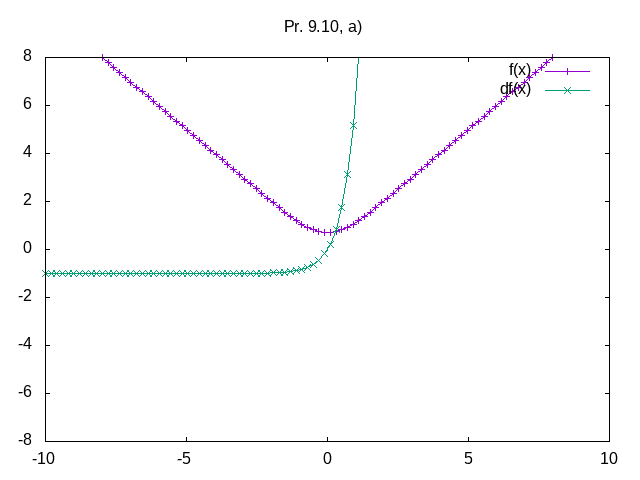
\includegraphics[width=.9\linewidth]{f1_1.1.png}
\end{center}

\subsection{b) \(f(x) = -\log(x)+x\)}
\label{sec:org7d159e4}

The first step puts us at x = -3, which \(f(x)\) is undefined on.
\begin{center}
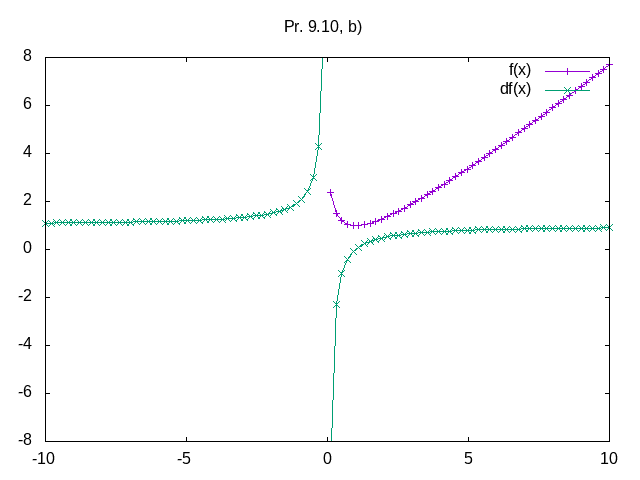
\includegraphics[width=.9\linewidth]{f2.png}
\end{center}
\end{document}